\namedsubsection{Sage}{J}
Wenn wir von Sage sprechen, ist stets das ERP System Sage 100 von gleichnamiger Softwarefirma gemeint. Die Version Sage 100 ist der Vorgänger der Versionen Sage 200 Evolution, Sage 300 Cloud und Sage X3 und ist sowohl als Cloud, als auch als lokale (On-Premise) Lösung verfügbar.

Im Kontext dieses Projektes haben wir uns ausschließlich mit der On-Premise Version befasst, da dieses auch bei dem Pilotkunden von Statistance lokal verwendet wird.

Das Sage System besteht aus folgenden Komponenten:

\begin{itemize}
  \item \textbf{Rich Client: } Das ERP System selbst ist als Rich Client Applikation implementiert, es wird also jegliche Applikationslogik im Prozess des Clients ausgeführt. Die Kommunikation zwischen Client und Applikationsserver findet über das Sage-eigene Protokol S-Data statt, welches im folgenden Kapitel ausführlich beschrieben wird.  Ein beispielhaftes User-Frontend ist in Abb.\ref{fig:sage_screenshot} zu sehen.

  \item \textbf{Applikationsserver: } 
  Da es sich um eine Rich Client Anwendung handelt muss der Applikationsserver für die Einhaltung der ACID Prinzipien, also insbesondere konsistente Datenhaltung kümmern. Daher entfallen auf ihn die zusätlichen Aufgaben der Isolierung einzelner Anwendungen für die parallele Ausführung und das Pooling von Applikationskernen \cite{sageadministrationshandbuch}.
  \item \textbf{Datenbank: } Als Datenbank wird eine MSSQL Datenbank verwendet, welche mindestens die Version \"Microsoft SQL Server 2008\" oder neuer verwendet.
\end{itemize}

\begin{figure}[!h]
\centering
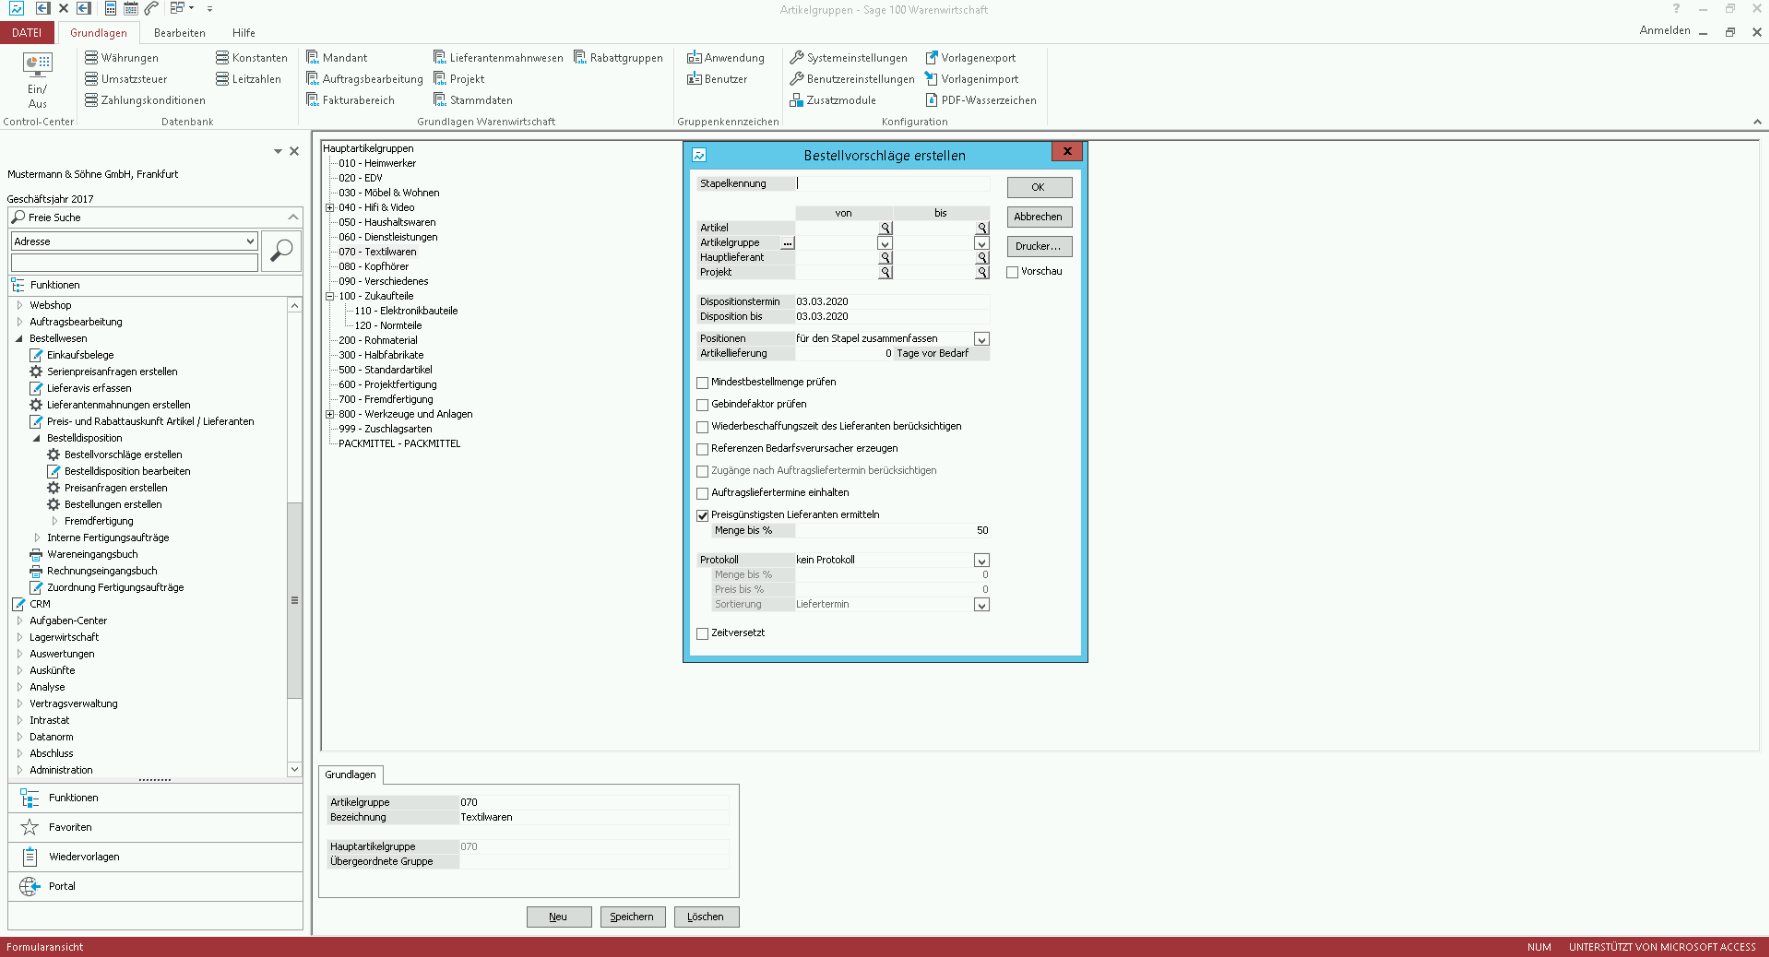
\includegraphics[width=13.5cm]{images/03_SAGE/Sage_100_Screenshot.png}
\caption{Rich Client Interface auf einem Windows Server}
\label{fig:sage_screenshot}
\end{figure}

\subsubsection*{Module}

Innerhalb des Sage 100 Systems existieren verschiedene Module, welche sich in die Kernmodule (Finanzwesen, Warenwirtschaft und Produktion) und Zusatzmodule einteilen lassen. Diese Module sind wiederum in Einzelbereiche aufgeteilt (z.B Einkauf und Verkauf). Für Statistance ist in diesem Kontext insbesondere der Einkaufsbereich des Warenwirtschaftsmoduls relevant, da dieser die Wareneingänge und Belege beinhaltet, für welche Sie ihre statistischen Vorhersagen treffen.

\namedsubsection{Sage 100 SData}{J}
Die SData Spezifikation beschreibt ein von Sage entwickeltes Protokoll zum lesen, ändern, erstellen und löschen von Daten aus dem ERP-System~\cite{sdatadocu}. Dieses Protokoll beschreibt den Aufbau der REST-Schnittstelle und wie die Kommunikation zwischen Consumer und Provider auszusehen hat. Die Daten werden hierbei in Form von Atom Feeds, ein Standard im XML-Format~\cite{atomfeed}, übertragen. Die Webservices für SData wiederum werden bei der Installation von Sage 100 automatisch mit installiert und sind standardmäßig aktiviert \cite{sageadministrationshandbuch}. Die Abbildung \ref{fig:sdataservicesadmin} zeigt hierbei alle aktiven SData Services bei einer Standardinstallation von Sage 100 an inklusive Anzahl der Zugriffe.

\begin{figure}[!h]
\centering
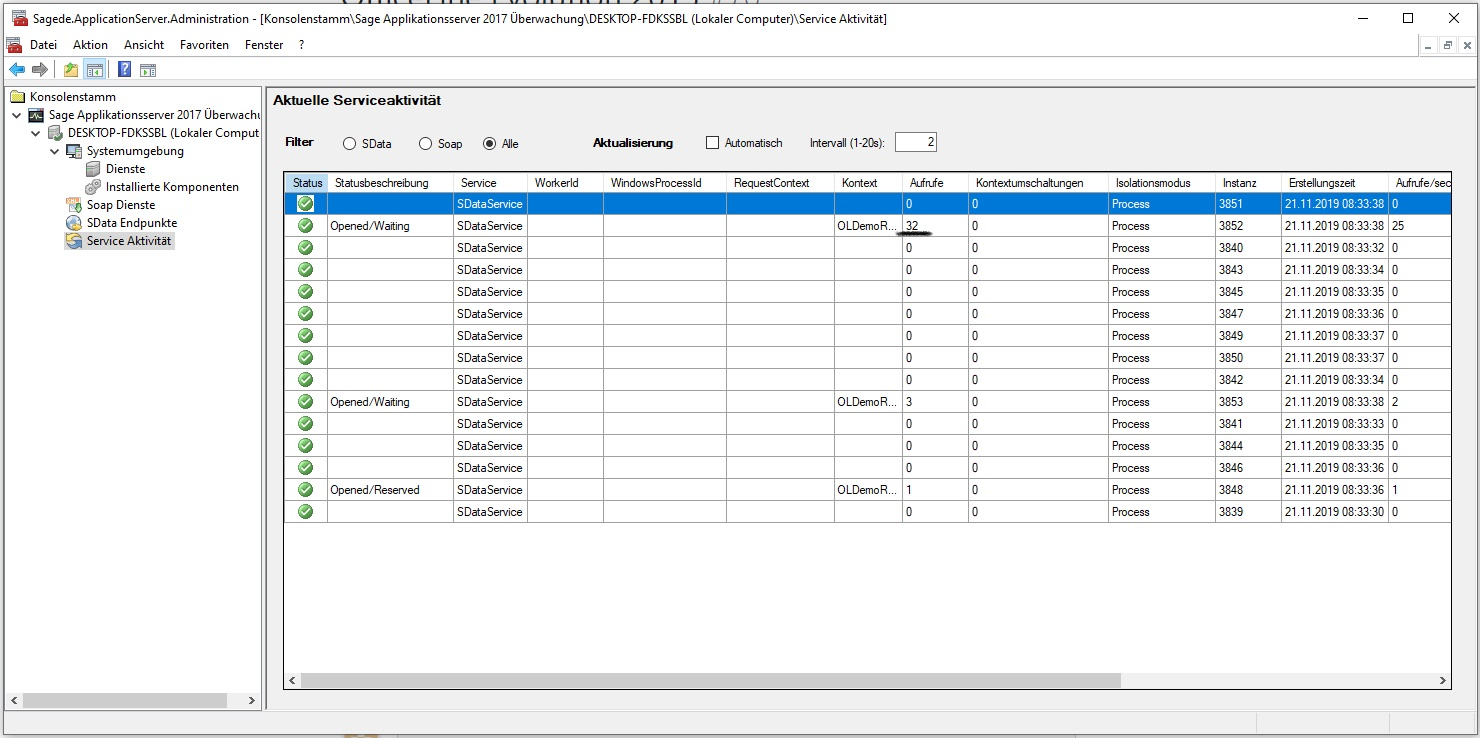
\includegraphics[width=12cm]{images/0x_requirement_analysis/sage-admin-sdata.png}
\caption{Adminpanel SData Services}
\label{fig:sdataservicesadmin}
\end{figure}

Interessant ist eine Untersuchung von SData für uns gewesen, weil es die Möglichkeit bieten könnte Daten sicher zurück in die Datenbank einzuspielen ohne sie fehlerhaft zu bespielen. Ebenfalls wäre die Schnittstelle eher für Fälle geeignet in denen die Dienste von Statistance als SaaS in Anspruch genommen werden. Bei einer Cloud-Lösung müssen Daten über das Internet übertragen werden. Das erstellen eines Adapters würde somit bei Nutzung von SData anteilig entfallen.

Die ursprüngliche Annahme ist gewesen, dass alle Endpunkte von SData grundsätzlich alle CRUD-Operationen erlauben. Dies fußte auf die initiale Begutachtung mehrerer Endpunkte bei denen das Löschen und Ändern der Daten problemlos möglich ist. Jedoch stellte sich diese Annahme nach Betrachtung der für uns wichtigsten Endpunkte später als Irrtum heraus.

* Beschreibung Aufbau Payload
** Attribute für Operatoren
** Beispielresponse

\begin{figure}[!h]
\centering
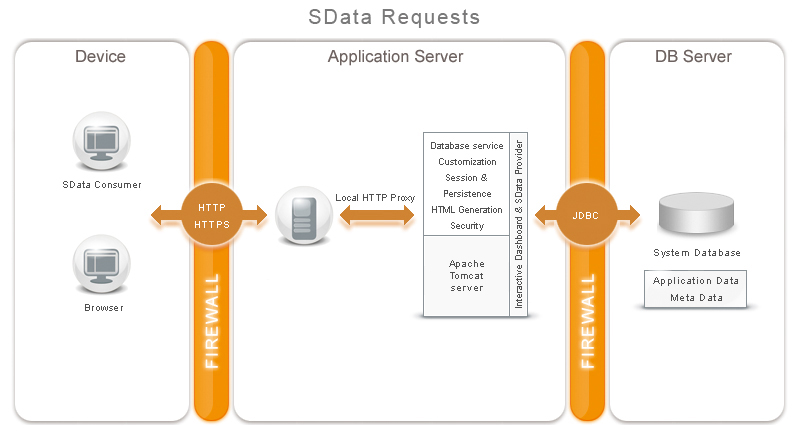
\includegraphics[width=12cm]{images/0x_requirement_analysis/sdata_requests_arch.png}
\caption{SData Integration in Sage~\cite{sdata_requests}}
\label{fig:sdataintegrationsage}
\end{figure}

Fehlermeldungen bei der ungültigen Nutzung der SData Services lassen darauf schließen, dass Sage intern verschiedene Safeguards für die Nutzung der Schnittstellen enthält um die ordnungsgemäße Funktionsweise der Datenbank zu gewährleisten. Auch eine Betrachtung der Integration von SData in den Applikationsserver von Sage bestätigen diesen Eindruck wie auf Abbildung \ref{fig:sdataintegrationsage} zu entnehmen ist.

\subsubsection*{Security}

Man hat die Möglichkeit die Authentifizierung entweder im Basic oder Digest-Modus auszuführen \cite{sdatadocu_auth}. Im ersterem Fall empfiehlt es sich den Datenaustausch mit SSL zu verschlüsseln weil die Login-Daten sonst sehr einfach auf dem Übertragungsweg abgegriffen werden können (z.B. über Man-in-the-Middle-Angriffe). Der andere Modus erfordert im Gegensatz dazu mehr Aufwand für die Umsetzung. Basic scheint in den vorhandenen Consumer-Clients enthalten zu sein. Beim anderen Modus ist es noch unklar.
Darüber hinaus findet sich im Handbuch die Erwähnung eines STS (Token Service) für SData, dass für die Absicherung von Verbindungen ebenfalls relevant sein dürfte \cite{sageadministrationshandbuch} (S. 51). Jedoch entsprechen diese Methoden nicht mehr den heutzutage empfohlenen Verfahren laut der OWASP \cite{owasp_authentication}.

Ebenfalls relevant ist die Autorisierung der Ressourcen. Über unterschiedliche Benutzerberechtigungen sollte es auch möglich sein den Zugriff einzuschränken bzw. auf Read-only zu setzen. Im Handbuch findet sich dazu eine Anleitung wie man den Zugriff je Benutzer auf bestimmte Bereiche beschränken kann \cite{sageadministrationshandbuch} (S. 33 f.).

\subsubsection*{Vorteile}
\begin{itemize}
    \item Es gibt bereits Consumer-Clients für C\# und JavaScript\footnote{Siehe https://github.com/Sage/SDataCSharpClientLib und https://github.com/Sage/SDataJavaScriptClientLib}
    \item REST-like Schnittstelle mit CRUD Capability
    \item keine direkte Datenbankanbindung nötig und “Bidirektional”
    \item Schemata können direkt vom Webservice abgefragt werden (Validierung)
    \item Die Schnittstelle ist auch Hypermedia-Driven, d.h. alle Daten werden immer mit navigierbaren Links ausgeliefert
    \item Automatisch SSL bei Installation \cite{sageadministrationshandbuch} (S. 22 und S. 26)
    \item Im Gegensatz zum direkten Datenbankzugriff Safeguards für das Löschen, Ändern und Hinzufügen von Daten vorhanden
\end{itemize}

\subsubsection*{Nachteile}
\begin{itemize}
    \item sehr wenig dokumentiert
    \item nicht alle Daten lassen sich erstellen
    \item Authentifizierung entspricht nicht mehr den heutzutage gängigen Standards \cite{owasp_authentication}
\end{itemize}

Wie man Einstellungen am SData Provider vornehmen kann ist im Handbuch dokumentiert \cite{sageadministrationshandbuch} (S. 57 ff., S. 36 f.).
Das Sage 100 ERP-System erlaubt es auch SOAP-Services zu installieren. Wie das abzulaufen hat kann unter Soap-Service Installation im Handbuch nachgesehen werden \cite{sageadministrationshandbuch} (S. 27).

\subsubsection*{Aufbau REST-API}
Alle Links beziehen sich momentan auf die derzeit laufende Demo-Instanz bei Statistance.
Aus uns noch nicht nachvollziehbaren Gründen antwortet der Linux Postman-Client auf eine Anfrage mit einer Server-Fehlermeldung. Es müsste in diesem Fall geklärt werden woran es genau liegt. Die Windows-Variante stellt keinerlei Probleme dar.

Meistens ausgehend von der baseurl 
\begin{quotation}
    https://app.statistance.de:5493/sdata/ol/Default/OLDemoReweAbfD;123
\end{quotation}
werden wir nachfolgend einige wichtige Endpunkte der SData Schnittstelle aufführen.

\begin{description}
    \item [https://app.statistance.de:5493/sdata/ol/Default]
    Enthält die Endpoint-URLs für die vorhandenen Datenbanken, in der Sage 100 Demo-Version werden jeweils zwei angelegt
Für uns erstmal relevant dürfte die URL zur Beispieldatenbank sein
ol steht vermutlich für Office Line
    \item [<baseurl>]
    Hier werden alle erreichbaren Endpunkte für die Beispieldatenbank aufgeführt
    Nachfolgend am Beispiel des Endpoints Adressen werden wir auf den groben Aufbau dieser Endpunkte eingehen. Der Aufbau ist für alle anderen Endpoints gleich.
    \item [<baseurl>/Adressen]
    Listet alle vorhandenen Adressen der Datenbank auf
    \item [<baseurl>/Adressen/\$schema]
    Enthält das XML Schema für Adressen
Zudem kann man anhand der Attribute sme:canGet(|Put|Post|Delete) im ersten xs:element-Tag erkennen was man mit der Ressource alles anstellen kann
    \item [<baseurl>/Adressen/\$template]
    Beispiel-Payload für zum Beispiel einem Put oder Post-Requests
    \item [<baseurl>/Adressen?where=\$updated gt @2019-12-19T22:00Z@]
    Mithilfe des where-Querys lassen sich Abfragen filtern
In unserem Beispiel sollen nur Adressen angezeigt werden die seit dem im @-Zeichen umschlossenem Datetime zuletzt geupdated wurde
Unglücklicherweise funktioniert das gegenwärtig nicht, weil das updated-Feld einer Ressource immer dem Requestzeitpunkt entspricht
Meiner Meinung nach kann das kein normales Verhalten sein, vielleicht lässt es sich in den Sage Einstellungen irgendwie beheben
Alle möglichen Operatoren, Funktionen und Spezialvariablen lassen sich in http://sage.github.io/SData-2.0/pages/core/0212/ einsehen
    \item [<baseurl>/Adressen?where=Adressen.ADR\_Gruppe eq 'MA']
    Ein weiteres Beispiel für die Nutzung des where-Querys
Query entspricht: Wähle nur Adressen aus die zur Adressgruppe der Mitarbeiter gehören
\end{description}